% Figure A4, generated by experiments/a4_raw_vs_refit.py.
\begin{figure}[t]
  \centering
  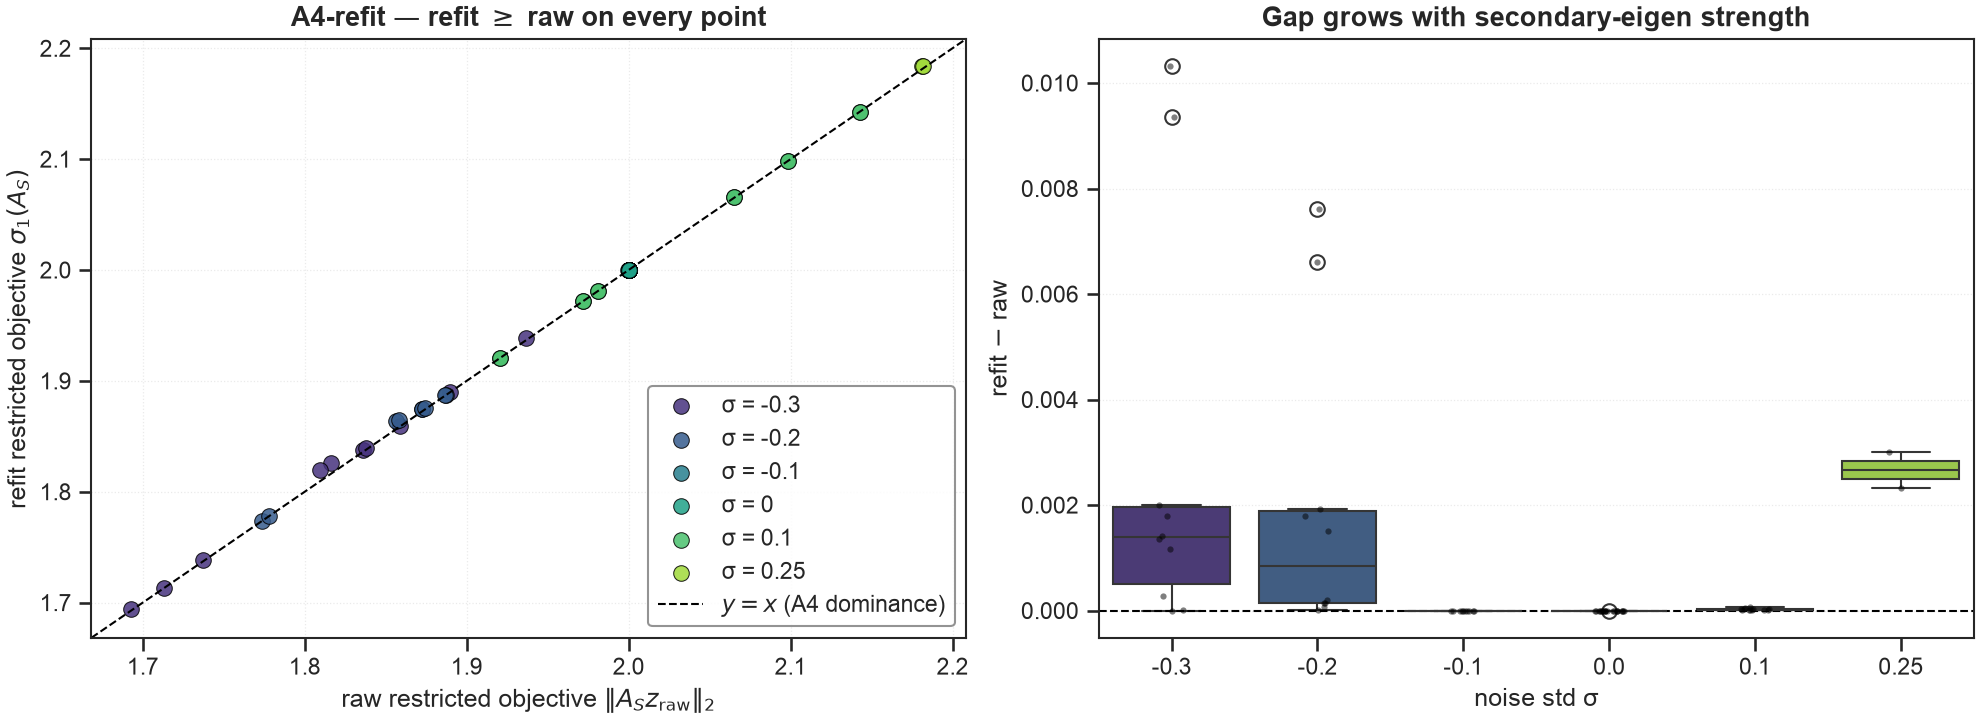
\includegraphics[width=\linewidth]{../shared/figures/generated/a4_raw_vs_refit.png}
  \caption{\textbf{A4-refit, restricted refit dominates raw selection.} Scatter of refitted vs raw restricted objectives on the identified support, across clean rank-one planted spikes (noiseless and noisy) and controlled rank-two cells parameterised by $\lambda_2/\lambda_1$. \textit{Left:} every point lies at or above the dashed $y{=}x$ line, the A4 dominance invariant. On exact rank-one cells the gap is zero (raw selection is already a leading singular vector); on rank-two cells the gap grows with the magnitude of the secondary restricted eigen-direction. \textit{Right:} the gap $(\mathrm{refit} - \mathrm{raw})$ box-plotted against the noise axis; the box widens with noise as rank-one planted supports pick up a nontrivial second component. Dominance pinned in \texttt{tests/test\_a4\_smoke.py}.}
  \label{fig:a4-raw-vs-refit}
\end{figure}
